
\documentclass[journal]{IEEEtran}
\usepackage{lmodern}
\usepackage{amsfonts}
%\usepackage{hyperref}

\usepackage{cite}
\ifCLASSINFOpdf
  \usepackage[pdftex]{graphicx}
  \graphicspath{{./img/}}
  \DeclareGraphicsExtensions{.pdf,.jpeg,.png}
\else
\fi
\usepackage{array}
\usepackage{url}
\hyphenation{op-tical net-works semi-conduc-tor av-er-age at-tribute}


\begin{document}
\title{Analysis of Genetic Algorithms Optimizing Topological Layout and Synaptic Weights }

\author{Taras~Mychaskiw(xxxxxxx)~\textless{}tm07qx@brocku.ca\textgreater\\%
Evan~Verworn~(4582938)~\textless{}ev09qz@brocku.ca\textgreater% <-this % stops a space
}

\maketitle

\begin{abstract}ah Blah Blah Blah Blah Blah Blah.
\end{abstract}

\IEEEpeerreviewmaketitle

\section{Introduction}
\IEEEPARstart{T}{his} should be written last. Blah Blah Blah Blah Blah Blah Blah Blah Blah Blah Blah Blah Blah. 

\section{Background}

% I don't think we'd have to write much on this and GAs. 
% I think about the same as a wikipedia summary.
  \subsection{Neural Networks}
  A high level description of a basic Neural Network is a single directional graph without cycles or reflexive edges. It is a mathematical model wherein given some number of inputs and some number of outputs, the outputs will react to the magnitude of the input values. A visualization is given in Figure \ref{fig:NeuralNetwork}.
  
\begin{figure}[here]%[!t]
  \centering
  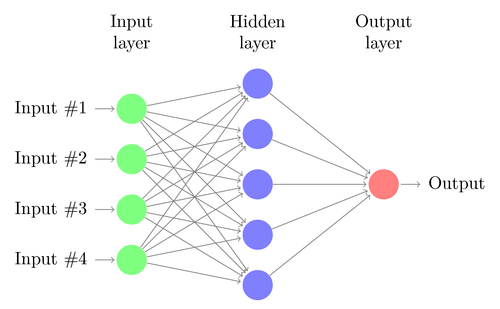
\includegraphics[width=3.4in]{neural-network}
  \caption{An example single hidden layer neural network.}
  \label{fig:NeuralNetwork}
\end{figure}

The output is \textit{trained} to the desired output through manipulating the weights in the intermediate (hidden) and output layer edges.  

\begin{figure}[here]
  \[  node\_output = \sum_{i=1}^{n} w_{i} x_{i} \]
  \caption{Where $n$ is the number of edges coming \textit{into} this node, $w$ is the weight associated with that edge and x is the output value produced by the predecessor node.}
  \label{fig:NodeOutput}
\end{figure}

A node calculates its output value by summing the output of all of its predecessors and multiplying that output by a weight assigned to that edge, this value is then squashed to a number traditionally between 0 and 1 by a Sigmoid function.

In the Figure \ref{fig:NeuralNetwork} there is only one hidden layer, but in our experiments we are evolving a network that can have up to three hidden layers. 

  \subsection{Genetic Algorithms}
  Genetic Algorithms or GAs are another mathematical model for finding an optimized solution in a large search space. This model is based off of Darwinian Evolution in that the best performing current solutions are bred together mixing genetic information from both parents into their children. These children are then evaluated, just as their parents were, and subjugated to the same breeding rules. 
  
  Like in biological evolution corruption of the genetic code can happen, this is a possibily destructive mutation that encourages diversity between parents. 
  %This sets this optimization technique apart from traditional hill climbers that don't introduce

In this experiment a GA is used to optimize the structure \amp weights of

\section{Methodology}
  \subsection{Mutations}
    Our custom mutations.
  \subsection{Crossovers}
    Our custom crossovers.

\section{Experiments}
  \subsection{Connect 4}
    Description of Connect 4 Problem
  \subsection{Quality of Wines}
    Description of Wines Problem
  \subsection{Experiment Setup}
    Parameters Used.
  
\section{Analysis}
Results

\section{Conclusion}
Things could have done better.

We believe this is due to crossovers used.

Blah-de-Blah.


% references section

% can use a bibliography generated by BibTeX as a .bbl file
% BibTeX documentation can be easily obtained at:
% http://www.ctan.org/tex-archive/biblio/bibtex/contrib/doc/
% The IEEEtran BibTeX style support page is at:
% http://www.michaelshell.org/tex/ieeetran/bibtex/
\bibliographystyle{IEEEtran}
% argument is your BibTeX string definitions and bibliography database(s)
%\bibliography{IEEEabrv,../bib/paper}
%
% <OR> manually copy in the resultant .bbl file
% set second argument of \begin to the number of references
% (used to reserve space for the reference number labels box)
\begin{thebibliography}{1}

\bibitem{SOM_KO}
Kohonen, T. (2001
Airs today: Monday
     90210
     Following, The
     Seed
     Tonight Show with Jay Leno, The
     Zero Hour (US)). Self-Organizing Maps. Third, extended edition. Springer, Berlin.

\bibitem{Dunn}
Dunn, J. (1974). "Well separated clusters and optimal fuzzy partitions". Journal of Cybernetics 4

\end{thebibliography}

% You can push biographies down or up by placing
% a \vfill before or after them. The appropriate
% use of \vfill depends on what kind of text is
% on the last page and whether or not the columns
% are being equalized.

%\vfill

% Can be used to pull up biographies so that the bottom of the last one
% is flush with the other column.
%\enlargethispage{-5in}



% that's all folks
\end{document}
